%Emma Callery's Senior Seminar Paper

\documentclass{sig-alternate}
\usepackage{color}
\usepackage{listings}
\usepackage{url}
\usepackage{natbib}

\begin{document}
\conferenceinfo{UMM CSci Senior Seminar Conference, December 2014}{Morris, MN}
\title{Static and Dynamic Types in Software Development}
\numberofauthors{1}
\author{
\alignauthor
Emma G. Callery\\
	\affaddr{Division of Science and Mathematics}\\
	\affaddr{University of Minnesota, Morris}\\
	\affaddr{Morris, Minnesota, USA 56267}\\
	\email{calle052@morris.umn.edu}
}

\maketitle

\begin{abstract}
The debate between statically and dynamically typed languages has been going on since dynamic types were first introduced. Arguments have gone back and forth for everything from the benefits of both to what makes programmers hate one type system or the other. Unfortunately most arguments made for and against both type systems tend to come from personal opinion or personal experience. 
This paper takes a look at several studies that tried to look at this debate empirically to determine if either type system has an actual benefit to programmers. The first study looked at how programmers prefer to incorporate types in their programs when they have the chose. Several studies compared the time required to write out similar code in both a static and a dynamic language. 
The results are quite surprising, there are times where a static type system are faster. While there are other times dynamic typed systems are faster and even times where there is no determinable winner. All of this ultimately suggests that there is no superior type system, it is mostly determined by the programmer.  
\end{abstract}

\keywords{Static Types, Dynamic Types, Programming Languages, Java, Groovy.}

\section{Introduction}\label{intro}
Type systems (see \citep{Pierce2002}) have played an important role in programming languages since the beginning. Type systems matter to everything from education to research to industry. And while a great number of educational programming languages are statically typed (e.g.,Java), a fair number of industry programs use a dynamic type system (e.g.,Groovy) for things like wed development. This leads to the question of "whether one system or another, either static or dynamic, has a larger benefit for the humans that use them"\cite{Mayer2012}. 

This question has lead to a large debate of the benefits and draw-backs to both type systems, with people arguing strongly for both sides. Several studies have been conducted to try to determine if any of the arguments given in favor of either type have any real support. 

This paper starts by defining what static and dynamic typed languages are in section \ref{types}, including arguments for both. Section \ref{programmers} looks at a study that analyzed past projects to find patterns in how programmers use types. Two more studies have tried to look for empirical evidence to support the claim the static is better, their studies and results are in sections \ref{benifits} and \ref{influence}. We try to draw together an answer to the big question in section \ref{results}.

\section{Background Information}\label{types}
The reason this debate 
The fault in many of these arguments is that most are not backed by empirical evidence but rather personal experience and opinions.

\subsection{Static Types}\label{static}
``A language is statically typed if the type of a variable is known at compile-time''\cite{NomeN2009}. For the type to be known at compile-time means that the programmer has \emph{declared} the type of the variable. Static languages compilers enforce these types by only allowing values of the declared type to be assigned to the variable. see Figure 1. This means that when the compiler goes through the code it not only checks other errors, but also checks for type errors.
 
\subsubsection{Arguments For Static Types}\label{arguments}
%\begin{itemize}
%\item Most error checking is done at compiled-time, therefore catching errors more quickly.
%\item Types help to communicate to the programmer and the programmer reason about the program.
%\item Requiring type names act as a form of documentation or improves the quality of the documentation.
%\item Improve the programs structure.
%\end{itemize}
Type checking is one argued benefits of static types. Since this checking is done at compile-time the errors are more likely to be caught quickly and without having to run the whole program as frequently. A second common argument is that types improve the structure of a program. Better structure is believed to help the programmer reason out the program. The last big argument for static types is that the types provide a form of documentation that can communicate to the programmer and others that read the program. With this documentation from the types added to the documentation written by the programmer will return greater quality documentation.

\begin{figure}
\centering
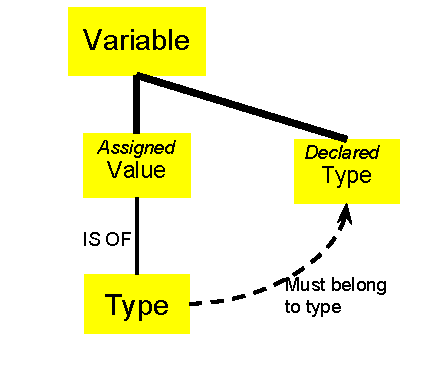
\psfig{file=Static_Type_Diagram.pdf,width =2in}
\caption{Diagram of Static Types \cite{Ferg2012}}
\end{figure}

\subsection{Dynamic Types} \label{dynamic}
``A language is dynamically typed if the typlookede of a variable is interpreted at run-time''\cite{NomeN2009}. This is because types in dynamic languages are only associated with values\cite{Pierce2002}.see Figure 2. This does not mean that a type can not be associated with a variable, only that the language would not require the type be declared. This \emph{option} leads to what is called \emph{optional typing} where the programmer is primarily  responsible for the types incorporated in the program, as explained in section \ref{programmers}. 

\subsubsection{Arguments For Dynamic Types}
%\begin{itemize}
%\item More flexible, variables can be passed between functions more easily.
%\item Without the need to declare every variable will make the program shorter, and therefore faster to write and read.
%\item Programs without specific type requirements can be easily reused, with out having to write a whole new function to do the same thing to a different type
%\item Not needing to declare variables, along with other 'administrative' commands, just to keep the compiler running allows for focusing to the conceptual concepts of the program.
%\end{itemize}
Not being required to type every variable is argued to make dynamic typed programs shorter and therefor faster to write and read. Dynamic types are also argued to allow greater flexibility to the programmer. There are several reason for this including easier passing of variables from different parts of a program. No specific type requirements allow for easier reuse-ability of part of programs. Declaring variables is considered 'administrative', so not needing to worry about keeping the compiler running would allow for focusing of more conceptual concepts of the program.

\begin{figure}
\centering
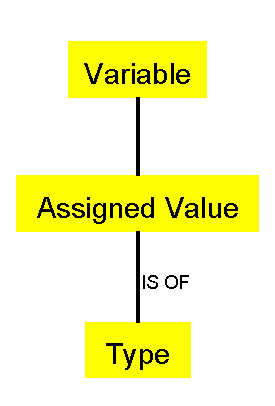
\psfig{file=Dynamic_Type_Diagram.pdf,width =1in}
\caption{Diagram of Dynamic Types \cite{Ferg2012}}
\end{figure}

\section{Programmer Preferences} \label{programmers}
This section will look at a study which attempted to determine where programmers use types and what types they used. The language used is the optional type language \emph{Groovy}. Groovy is actually dynamically typed language, but can access the static types in Java, and claims to "seamlessly integrate with existing Java classes" \cite{Souza2014}

\subsection{Study on Optional Typing}
Carlos Souza and Eduardo Figueiredo tried to understand programmer preferences in their paper \emph{How do Programmers Use Optional Typing? An Empirical Study}. In this study Souza and Figueiredo looked at 6638 projects written in the language Groovy. Looking over all of the projects Souza and Figueiredo tried to answer several questions about the use of types in the different projects. The questions were: 
\begin{enumerate}
\item \label{interface} ``Do programmers use types more often in the interface of their modules?''
\item \label{tests} ``Do programmers use types less often in test classes and scripts?''
\item \label{experience} ``Does the experience of programmers with other languages influence their choice of typing their code?''
\item \label{sizeageactivity} ``Does the size, age or level of activity of a project have any influence on the usage of types?''
\item \label{changed} ``In frequently changed code, do developers prefer typed or untyped declaration?'' 
\end{enumerate}
After collecting data from all the projects Souza and Figueiredo sorted the data by different measures; like the kind of type declaration, the usage of types, the size of the project in lines of code, the age of the program. It was from this data and different comparisons that Souza and Figueiredo attempted to answer their questions.

\subsection{results of optional typing}
Question \ref{interface} was found to be true; variables and fields that are public, such as constructor parameters, are frequently typed. Though the reason for why module definitions are most often typed is still unresolved, Souza and Fiqueiredo suggest that the implicit documentation the types provide are the main incentive as programmers may consider documentation in these area important.

On the other hand, Question \ref{tests} was found to be false. Documentation is rarely needed for test classes and scripts as most are small and easy to understand already. Test classes tend to have one sole purpose, and are very rarely reused. While scripts can't be accessed by other modules so the type being passed is most likely already known. 

Unsurprisingly, question \ref{experience} was true. How a programmer uses types in an optional language greatly reflects how that programmer types in other languages. Programmers coming from a statically typed language are more likely to add types than a programmer coming from a dynamically typed language. It has been found that programmer become comfortable in what ever language they use most frequently.

While Souza and Figueiredo ``initially believed that,[as time goes on and the projects grows], the maintenance of projects becomes more difficult, leading programmers to use more types as a means to make code more readable''. The data gathered to try to answer question \ref{sizeageactivity} however showed that this was not the case. Souza and Figueiredo thought that maybe the data they gathered could not ``actually correlate to the need for maintenance'' or if the data could work ``programmers might not have the opportunity of desire to make their code more maintainable''.

Question \ref{changed} probably has the biggest debate attached to it. Some argue that type, acting as a form of documentation, could make frequently changed code easier to change. However untyped code, being simpler, can be changed faster. It's this later argument that Souza and Figueiredo found evidence for. They found that as changes in a file increase in frequency the use of untyped declarations also grows.

Overall this means that programmers are influenced by the types system that their use to. Though generally, programmers mostly type the definitions of a modules interface more frequently then anything else. Programmers also tend to drop types when they have to keep making changes to pieces of code. However this means that this debate of static vs dynamic needs to be looked at more closely to determine if there is an actual benefit to one type system over the other. For this the two paper discussed in the following sections attempted to prove that static types are better. 

\section{Influence of Static Types}\label{influence}
This section looks at a study conducted by Stefan Hanenberg, Clemens Mayer, Romain Robbes, Andreas Stefik, and Eric Taner in their paper \emph{An Empirical Study of the Influence of Static Type Systems on the Usability of Undocumented Software}\cite{Mayer2012}. This study looked into the argument that types act as a form of documentation. Arguing that if there is no other form of documentation present and variables are not typed, it should take a programmer longer to complete a task then if the variables are typed. 

The researcher hypothesized that ``the development time for completing a programming task in an undocumented API is equivalent when using either a static type system of a dynamic type system.''\cite{Mayer2012} Because this hypothesis only accounts for the design of the API as a whole, hypothesis two was included. Hypothesis two states that "there is no difference in respect to development time between static and dynamic type systems, despite the number and complexity of type declarations in an undocumented API. Both were used so that if either hypothesis is rejected by the data insight can be gained on the relative benefits and consequences of both type systems. 

The experiment designed for this study had 27 subjects that had  experience with the chosen static language, Java, but had no experience with the chosen dynamic language Groovy, which had needed to be restricted to be a purely dynamic equivalent to Java. Subjects were separated into two groups, each group was asked to complete five distinct programming tasks in one language using an undocumented API before completing five similar tasks in another language with another API. Group one would complete the first assigned tasks using Java and then complete the next five tasks using Groovy. The other group did the same sets of tasks in reversed. The tasks were designed to vary in difficulty and the number of type declarations required.

It should be noted that the dynamic API was made by taking the static API and removing the type annotation. This posses a problem in that this does not use any of the possible features of dynamically typed languages. 

Also interesting to note is that one subject was removed from the experiment because it was found that the subject had ``spent a very large amount of time in reading the complete source code while working on task 2 and then solved tasks 3 and 4 quickly''\cite{Mayer2012}. After this had been confirmed to be the case and that it was the way the subject worked the subjects data was removed. This just confirms that different programmers have different ways of processing and writing code, meaning that there is no one way of programming that could work for everyone. 

\subsection{results}
\begin{figure}
\centering
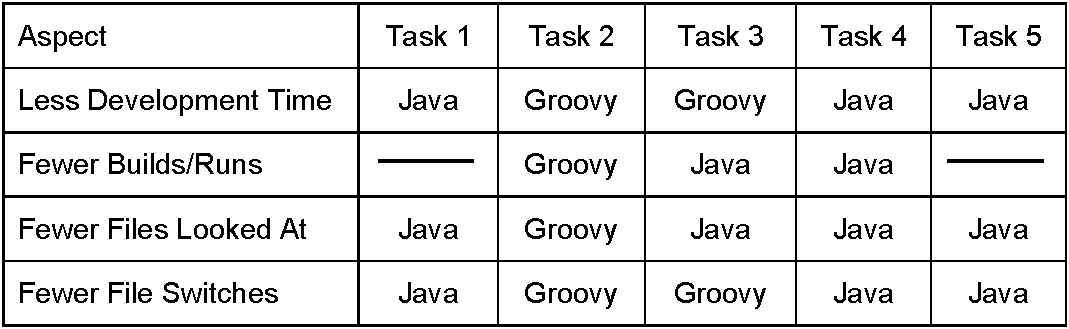
\psfig{file=Influence_Paper_Results.pdf,width =3in}
\caption{All results for all test(directly from paper)\cite{Mayer2012}}
\label{influenceResults}
\end{figure}
After analysis if the collected time data it was found that, concerning the first hypothesis, three tasks showed a positive impact for Java while the other two showed a positive impact for Groovy, as seen if Figure \ref{influenceResults}. This caused hypothesis one to be rejected, but hypothesis 2 cannot be rejected because the just the number and difficulty of the types ``cannot be a main effect of the difference between static and dynamic''\cite{Mayer2012}.

The contrary nature of the results lead to an investigation to find if other factors could be caused by other factors. One suggested factor was the number of builds and times tests were run during each task. These numbers were taken from the times the compiler ran and the times the 'start-button' was clicked. Two tasks registered no significant difference between Java and Groovy in number of builds and tests run. Another two tasks showed that the language with the shortest time also had the fewest test run. The surprising result was that one task had flipped results, Groovy had the shortest time while Java had been run less. 

A second suggested factor was the number of files the subject was looking at, which may indicate the amount of the source code that needed to be read in order to complete the task. This  could have an effect in that subjects using the dynamic system may be more likely to look at unrelated source code. Evidence gathered seems to support this theory for all but one task. For four of the five tasks fewer files were watched when the subject was using Java.

One final suggested factor was that the times the subject switched could indicate the amount of exploration the subject did while solving the task. Similarly to the previous suggestion, the effect would come from the need for user of a dynamically typed language to frequently change files to find or formulate answers. This was done separate from the previous analysis. Oddly enough the results from this analysis directly correspond to the development time results, for each task. This suggests that the number of switched files could be an indicator for the resulting development time. 

\section{Static Vs Dynamic Type Systems}\label{benifits}
This section discusses the study and results of Andreas Stuchlik and Stefan Hanenberg's study \emph{Static vs. Dynamic Type Systems: an Empirical Study About the Relationship between Type Casts and Development Time}\cite{Stuchlik2011}. The study was designed for the argument that in pure programming tasks the existence of type declarations leads to a reduction of development speed. Reasoning being that including type declarations should lead to better development times, through types improving the program structure and the programmers understanding.

The study had 21 subject, who were asked to complete five programming tasks in both Java and Groovy, where Groovy was in a similar restricted state as in the study above. Also like the study above, the subjects were split into two groups; one group started in Groovy then completed the same tasks in Java, the other group did the reverse. It should be noted that all subjects were familiar with Java, but none had used Groovy. All subjects were given two similar applications, consisting primarily of a data model, with five task associated with that application. One application would be completed in Java the other in Groovy.


Though the number of declarations did match between applications, each of the five tasks with in an application had varying numbers of type declarations required to successfully pass the associated tests. The assumption in this being that ``the higher the number of type [declarations] is, the larger is the difference in development times for the statically of dynamically typed code.''\cite{Stuchlik2011} Each task also varied on the minimum number of lines of code required to write out the code. Important to note however is that all the tasks are trivial, being neither complex nor requiring any other software, like an API. 
 
\subsection{results}
The results of this study were rather interesting in that there was no measured benefit from the static type system for any of the five tasks in either group. While the group that started in Groovy had only one task that showed a measurable positive impact of Groovy, the group that started in Java showed a positive impact in that task as well as one other task and in the overall time. When the results of both groups were combined, Groovy was found to have a measurable positive impact on three of the five tasks as well as in the total time. For the other two tasks no measurable difference could be found.

To try and understand the results another way Stuchlik and Hanenberg decided to sort the subjects between being 'outperforming' and 'underperforming' Java users. By this separation they hoped to determine if the results differed among the subjects in both groups. These results showed that with in the outperforming subjects a positive impact of Goovy could only be found in one task while the other four, and the overall time, registered no significant difference. The underperforming subjects however showed the same results as the combined groups.

It should be noted that these results only concern trivial programming tasks, and would not apply to non-trivial task. Which is the argument the authors give as to why this study should in fact weaken the arguments in favor of dynamic type system. They argue that ``as soon as we speak about non-trivial programming tasks, no positive impact can be measured'' though they do not point to a study that could actually answer that that statement.

\section{Threats of Validity}
maybe?

\section{Conclusions}\label{results}
This argument will probably never end. There will always be people that believe that one type system is better than the other and are unwilling to change their minds or how they program. Static types seem to be more beneficial in academia where students need to be able to understand the reasoning of code and the format it's written in. However, the web development industry probably couldn't care if anyone besides them understands the code. Ultimately, I think this argument will never go away because, but unlike politic, majority does not always rule.

\section{Acknowledgments}


\bibliographystyle{abbrv}
\bibliography{My_paper.bib}


\end{document}
